\documentclass[tikz,convert={density=300,outfile=\jobname.png}]{standalone}
\usepackage[utf8]{inputenc}		% bei der Verw. von lualatex oder xelatex entfernen!
\usepackage{tikz}

\usetikzlibrary{positioning}

\begin{document}
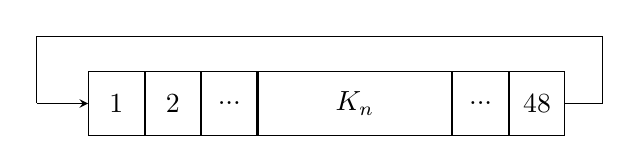
\begin{tikzpicture}

\node[draw, minimum width=70pt, minimum height=23pt] (main) {$K_n$};
\node[draw, minimum width=20pt,minimum height=23pt, right=0pt of main.east, anchor=west] (r1) {...};
\node[draw, minimum width=20pt,minimum height=23pt, left=0pt of main.west, anchor=east] (l1) {...};

\node[draw, minimum width=20pt,minimum height=23pt, left=0pt of l1.west, anchor=east] (l2) {2};
\node[draw, minimum width=20pt,minimum height=23pt, left=0pt of l2.west, anchor=east] (l3) {1};
\node[draw, minimum width=20pt,minimum height=23pt, right=0pt of r1.east, anchor=west] (r2) {48};

%set anchor points for the path
\node[right=10pt of r2.east] (anch1) {};
\node[above=17pt of anch1] (anch2) {};
\node[left=15pt of l3.west] (anch4) {};
\node[above=17pt of anch4] (anch3) {};

\draw (r2.east) -- (anch1.center) -- (anch2.center) -- (anch3.center) -- (anch4.center);
\draw[->	,>=stealth, scale=2] (anch4.center) -> (l3.west);
\end{tikzpicture}
\end{document}